% arara: closeAR
% arara: pdflatex
% arara: pdflatex
% arara: showfile
\documentclass[aspectratio=169]{beamer}

\usepackage{tikzlings}
\usetikzlibrary{positioning}
\usetikzlibrary{intersections}
\usetikzlibrary{backgrounds} 
\usetikzlibrary{decorations}
\usetikzlibrary{decorations.pathmorphing}
\usetikzlibrary{decorations.shapes, shapes.geometric}
\usetikzlibrary{decorations.markings}

\colorlet{mycyan}{cyan!30!white} 
\colorlet{myorange}{orange!70!yellow} 
\colorlet{myyellow}{orange!45!yellow} 
\colorlet{mygreen}{green!70!blue} 
\colorlet{mybrown}{brown!75!black} 

\setbeamertemplate{navigation symbols}{}
\setbeamertemplate{background canvas}{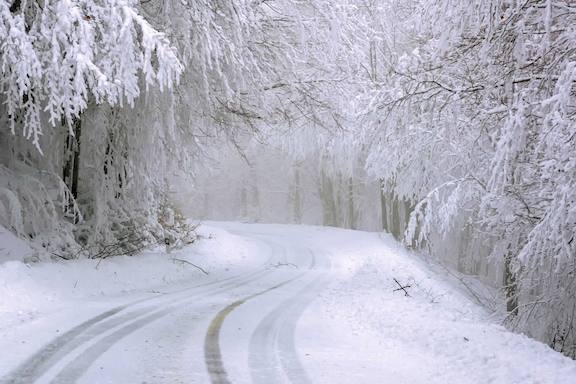
\includegraphics[width=\paperwidth]{strada.png}}

% trick taken from https://topanswers.xyz/tex?q=1989
\tikzset{
    use page relative coordinates/.style={
        shift={(current page.south west)},
        x={(current page.south east)},
        y={(current page.north west)}
    },
}

\usepackage{xfp}
\ExplSyntaxOn
\let\intmodnn\int_mod:nn
\ExplSyntaxOff

\newcommand{\isopen}{%
\ifnum \intmodnn{\thepage}{20} > 10
  _left
\else
  _right
\fi
}

\begin{document}
\begin{frame}
  \def\steps{500}
  \begin{tikzpicture}[remember picture, overlay,use page relative coordinates]
     % credit for background image
    \node[black,text width=.7\paperwidth,font=\tiny,align=center] at ([yshift=0.35cm]current page.south) {Image source: \href{https://pixabay.com/photos/road-trees-snow-cold-ice-frost-4730553/}{https://pixabay.com/photos/road-trees-snow-cold-ice-frost-4730553/}};
  \end{tikzpicture}
  \begin{tikzpicture}[remember picture, overlay,]
    \draw[decorate,
      decoration={markings,
      mark=at position .7*\thepage/\steps
      with {
        \node[anchor=south, transform canvas={scale=.7+\thepage/\steps}] {\includegraphics[page=1]{funny_marmots\isopen}};
        \node[anchor=south,xshift=2cm, transform shape={scale=.7+\thepage/\steps}, transform canvas={scale=.7+\thepage/\steps}] {\includegraphics[page=2]{funny_marmots\isopen}};
        \node[anchor=south,xshift=4cm, transform shape={scale=.7+\thepage/\steps}, transform canvas={scale=.7+\thepage/\steps}] {\includegraphics[page=3]{funny_marmots\isopen}};
        \node[anchor=south,xshift=6cm, transform shape={scale=.7+\thepage/\steps}, transform canvas={scale=.7+\thepage/\steps}] {\includegraphics[page=4]{funny_marmots\isopen}};    
      }}]
      (6,-4) to[out=-10, in=0] (-3,-2.9);
     \end{tikzpicture}
  \pause[\steps]
\end{frame}  
\end{document}